\section{Morphology}
\label{section:morphology}
Morphological operations are yet another set of neighborhood operators however unlike filtering they are designed to modify the shape of objects in binary images specifically. Producing a binary image from a coloured one involves first converting that image to grayscale and then thresholding (Equation \ref{eq:threshold}) its intensity such that pixels are converted to a 1 or 0 depending on whether they lay above or below the threshold (Figure \ref{fig:thresholding}). These are useful operations when you wish to modify an object's shape in order for it to fit some criteria, for example its total area or whether or not it's an open or closed contour. All morphological operators work by convolving a binary \emph{structuring element} with an image and thresholding the output pixel. There are two fundamental morphological operations, \emph{dilation} and \emph{erosion}, that comprise all others. 

\begin{figure}[htbp]
    \centering
    \begin{subfigure}[b]{0.3\textwidth}
        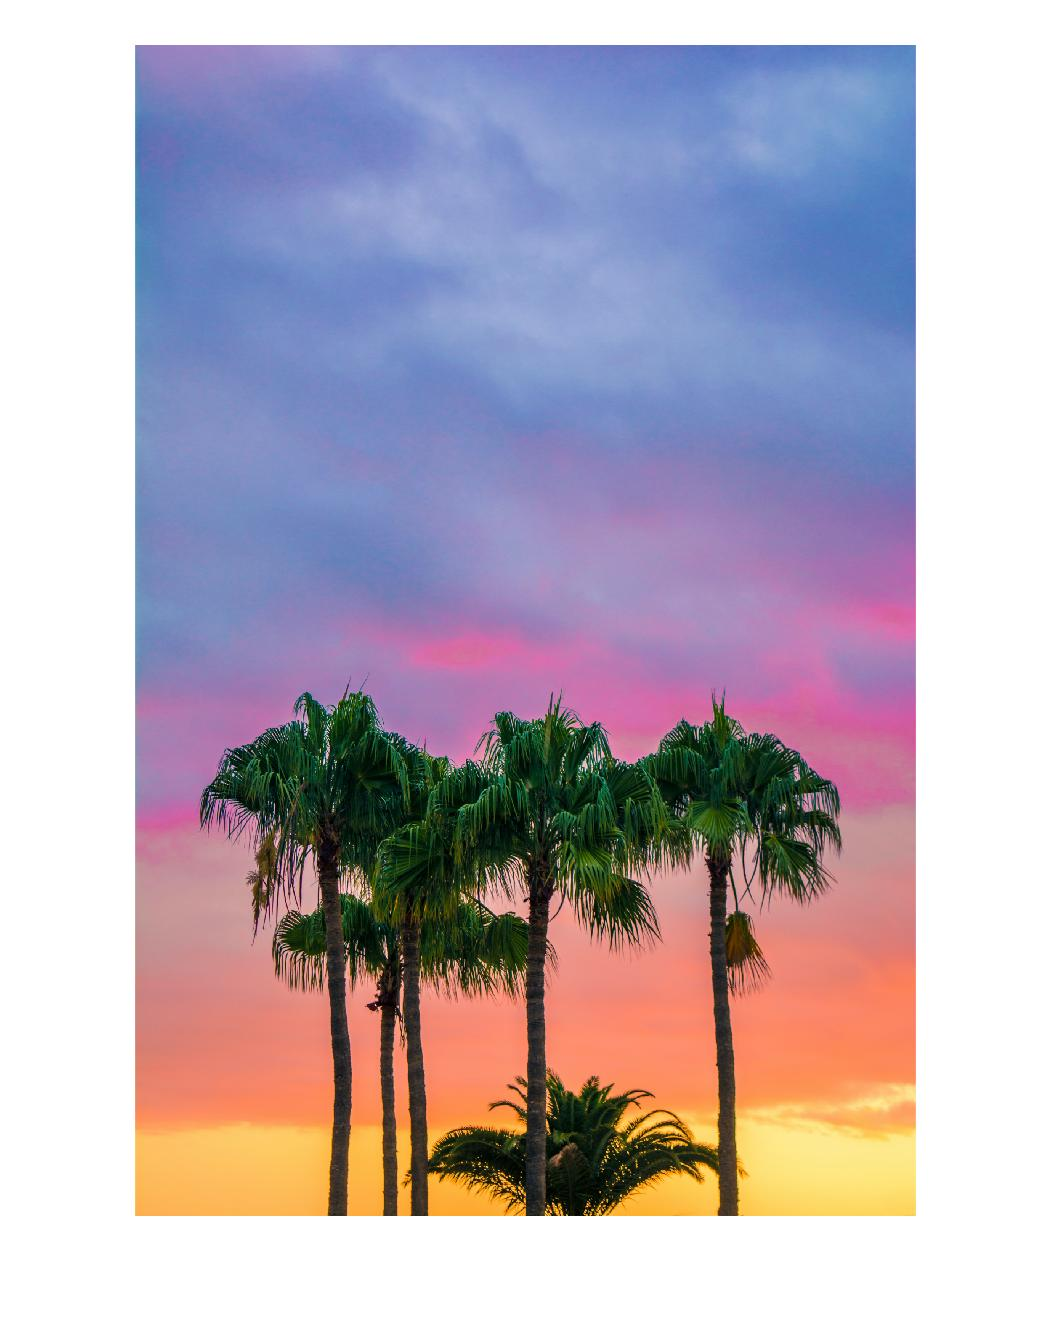
\includegraphics[width=\textwidth]{palms_resized}
        \caption{RGB Image}
        \label{fig:emu_noise}
    \end{subfigure}
    \begin{subfigure}[b]{0.3\textwidth}
        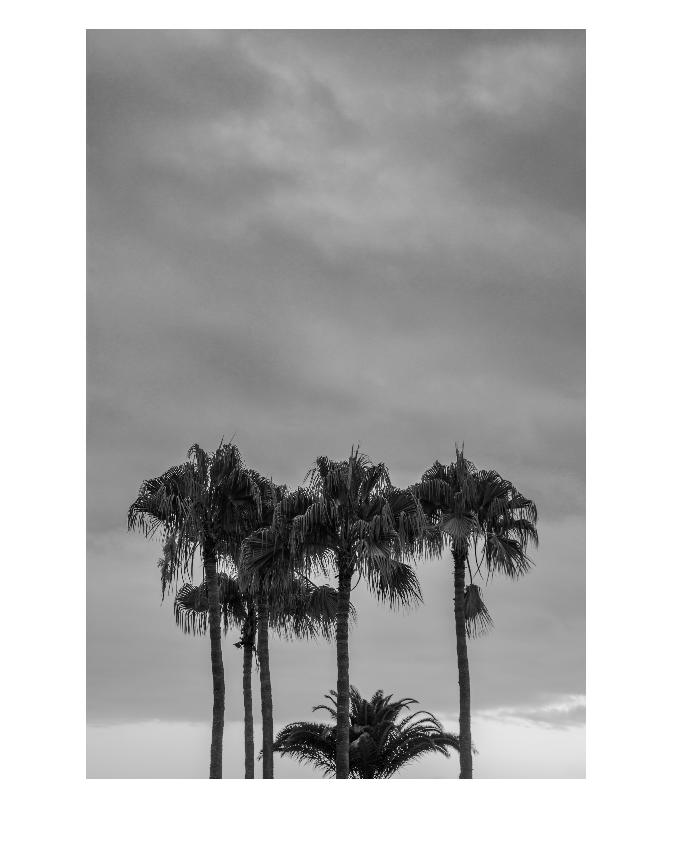
\includegraphics[width=\textwidth]{palms_grayscale}
        \caption{Grayscale Conversion}
        \label{fig:emu_gauss}
    \end{subfigure}
    \begin{subfigure}[b]{0.3\textwidth}
        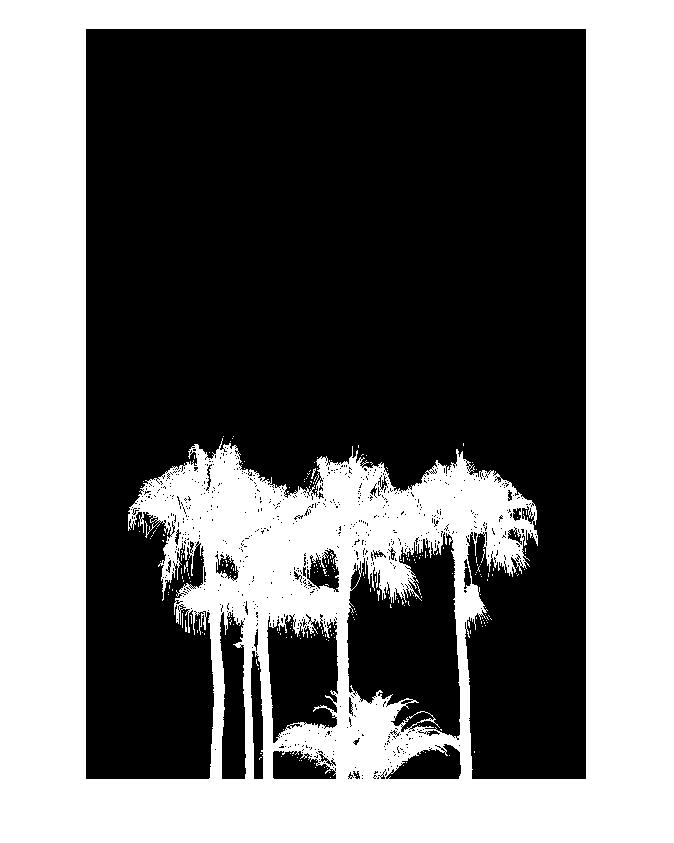
\includegraphics[width=\textwidth]{palms_binary}
        \caption{Binary Thresholding}
        \label{fig:emu_median}
    \end{subfigure}
    \captionsetup{format = hang}
    \caption{Conversion of an RGB image to a binary image. Original image by Adam Birkett}
    \label{fig:thresholding}
\end{figure}



\subsubsection{Dilation}

Dilation fills out or enlarges an object in a binary image in a way that is characterised by the specific structuring element used for the operation. A structuring element itself is just a binary image, generally a lot smaller than the target image itself, of a similar nature to a filter kernel, having an origin or reference pixel at thei center. In Figure \ref{fig:ice_dilation} the dilation causes objects to fill in gaps and even small spurious objects are inflated. This is because the structuring element \ref{fig:structuring_element} is simply a 9x9 pixel square where each convolution of the filter with the image outputs a 1 if the element overlaps at least one pixel of a binary object. This is a useful operation for filling in gaps in objects or thickening lines.


\subsubsection{Erosion}

Erosion performs the opposite function to dilation causing objects to contract rather than grow. Again, the structuring element is convolved with a binary image but and the output is placed at the structuring element's origin in the resulting image. Intuitively, wherever the structuring element is not completely inside an object the output is stored as black. In Figure \ref{fig:morphology} the structuring element we see that many smaller entities are erased from the image and many salient features are removed from large objects. This has the effect of 'cleaning up' the binary image of all speckle and spiky features, the nature of the cleanup depends on the size and shape of the structuring element, in this case the structuring element (\ref{fig:structuring_element}) is a simply square of size 9, so it acts like an eraser wiping anything that's approximately the same size or smaller.


\subsubsection{Opening and Closing}

Opening and closing are composite operations comprised of an erosion and dilation, each of which may use the same or different structuring element. An opening is an erosion followed by a dilation which is usel for isolating and cleaning up objects that might be just 'kissing' by first removing entities that are probably too small to be of interest, refining of object edges and breaking of thin connections and then smoothing of the remaining objects. In Figure \ref{fig:ice_open} it can be seen that many spiky entities are removed and some thin connection broken creating discrete objects that are smooth in somewhat thicker. Closing is the opposite ordere operation to opening performing first a dilation then an erosion. This is useful is you want to join objects together and preserve objects that might have been wiped out by an initial erosion. In Figure \ref{fig:ice_close} it can be seen to close many small gaps between objects and fill them in but still result in smooth large objects as a consequence of the erosion. Therefore, an opening can be thought of as useful for separating objects from one another and closing is good at joining them together. 

\renewcommand{\arraystretch}{0.6} % because \baselinestretch is 1.6667
\begin{figure}[H]
    \centering
    \begin{subfigure}[b]{0.49\textwidth}
        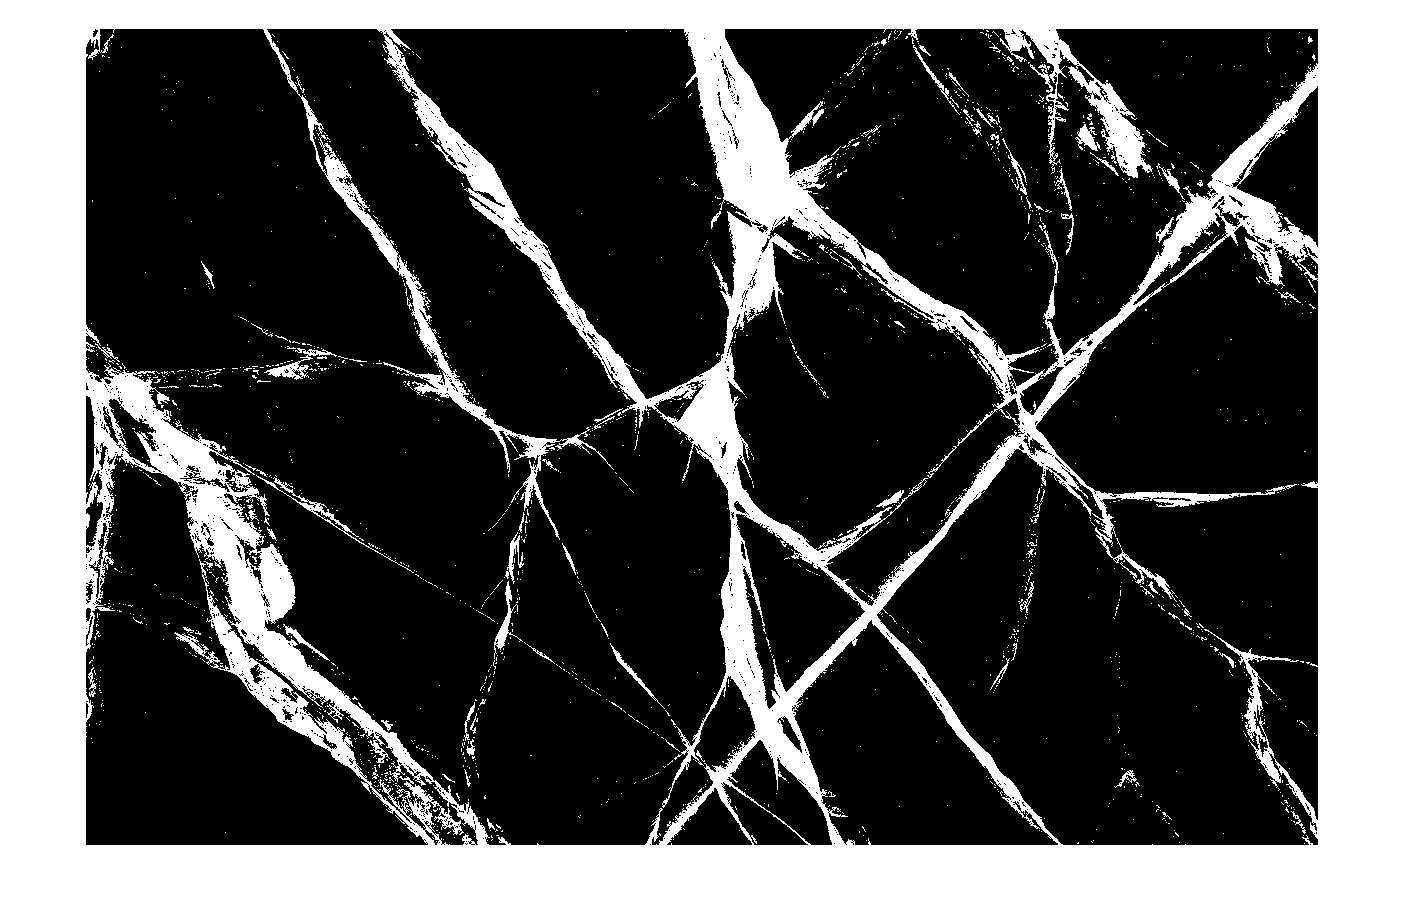
\includegraphics[width=\textwidth]{ice_binary}
        \caption{Binarized image}
        \label{fig:ice_binary}
    \end{subfigure}
    \begin{subfigure}[b]{0.49\textwidth}
        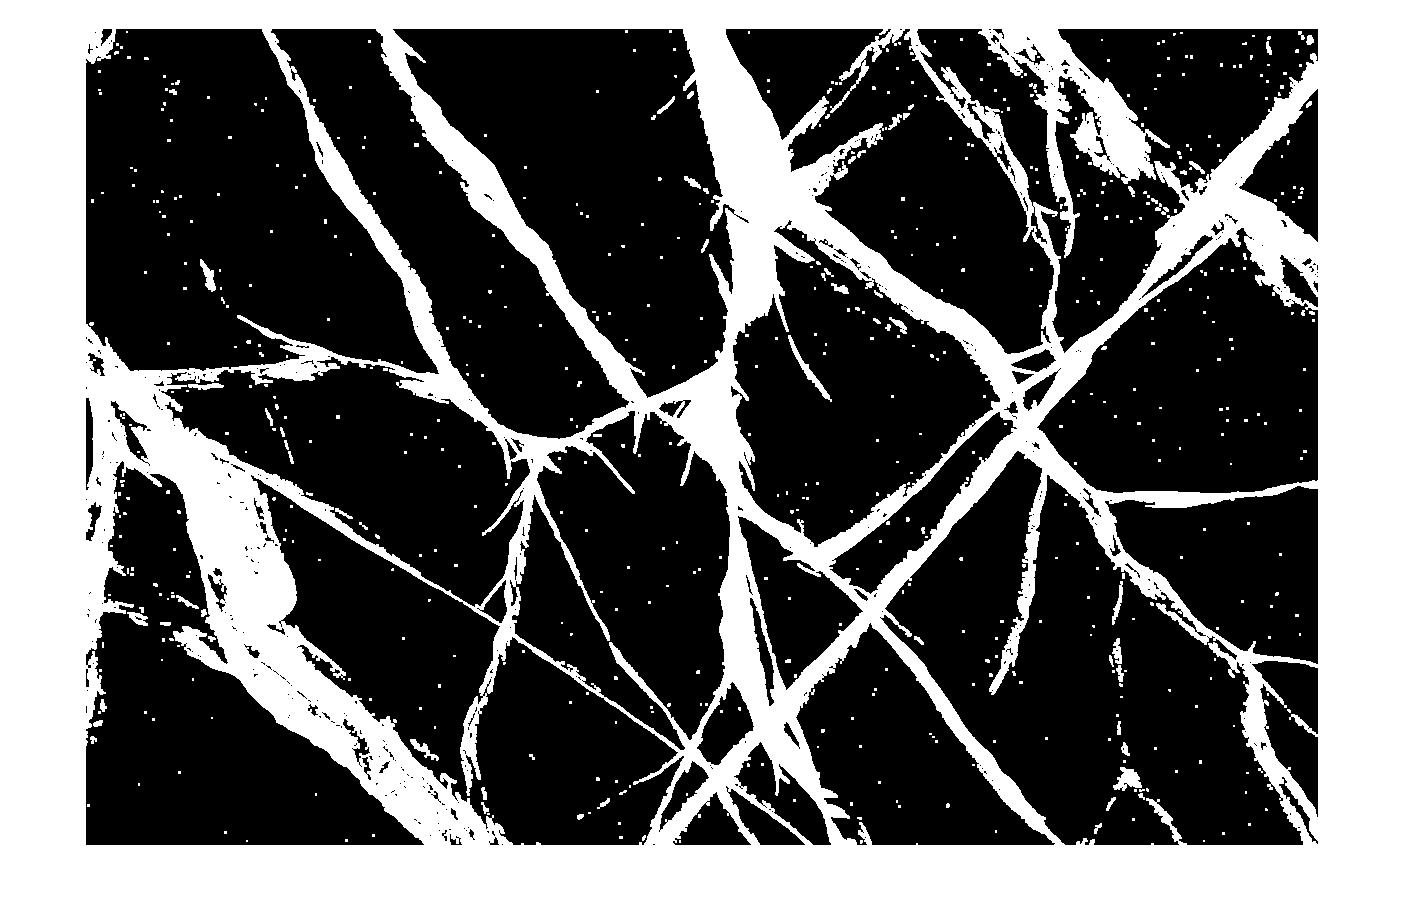
\includegraphics[width=\textwidth]{ice_dilate}
        \caption{Dilation}
        \label{fig:ice_dilation}
    \end{subfigure}
    \begin{subfigure}[b]{0.49\textwidth}
        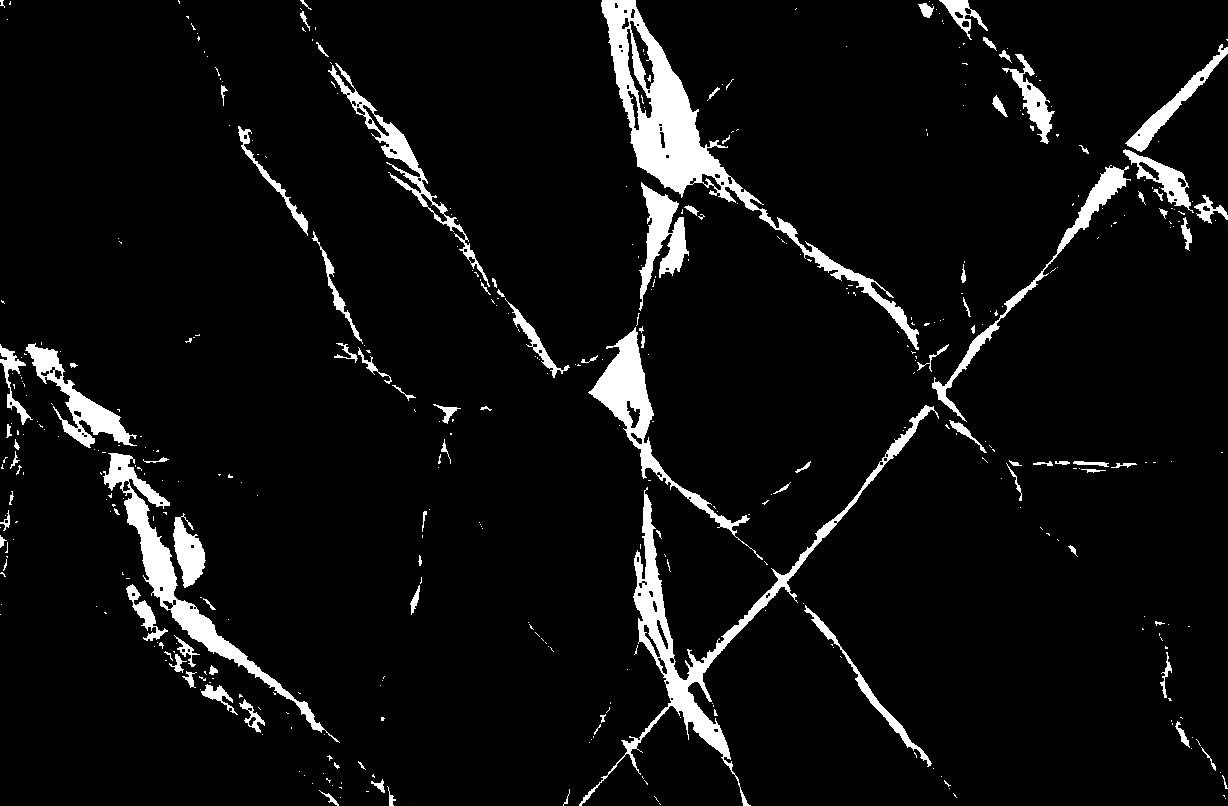
\includegraphics[width=\textwidth]{ice_erode}
        \caption{Erosion}
        \label{fig:ice_erosion}
    \end{subfigure}
    \begin{subfigure}[b]{0.49\textwidth}
        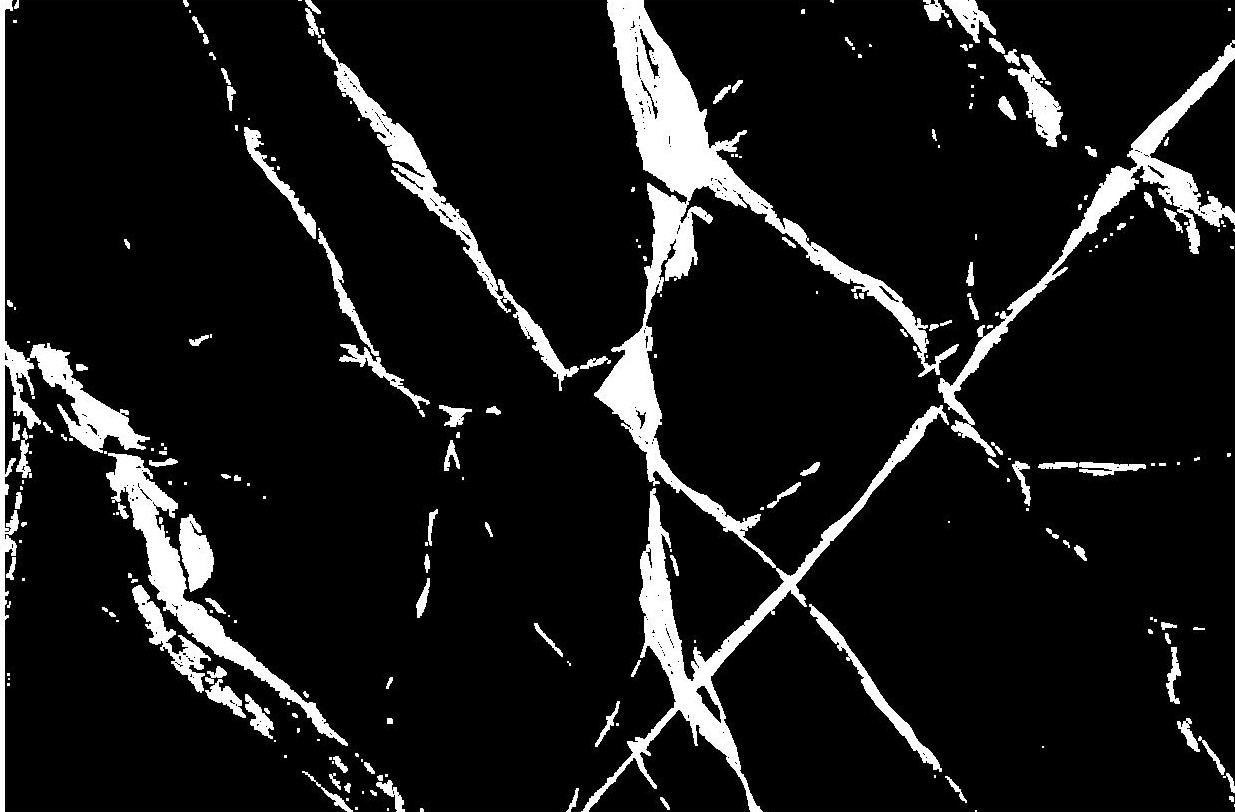
\includegraphics[width=\textwidth]{ice_open}
        \caption{Opening}
        \label{fig:ice_open}
    \end{subfigure} 
    \begin{subfigure}[b]{0.49\textwidth}
        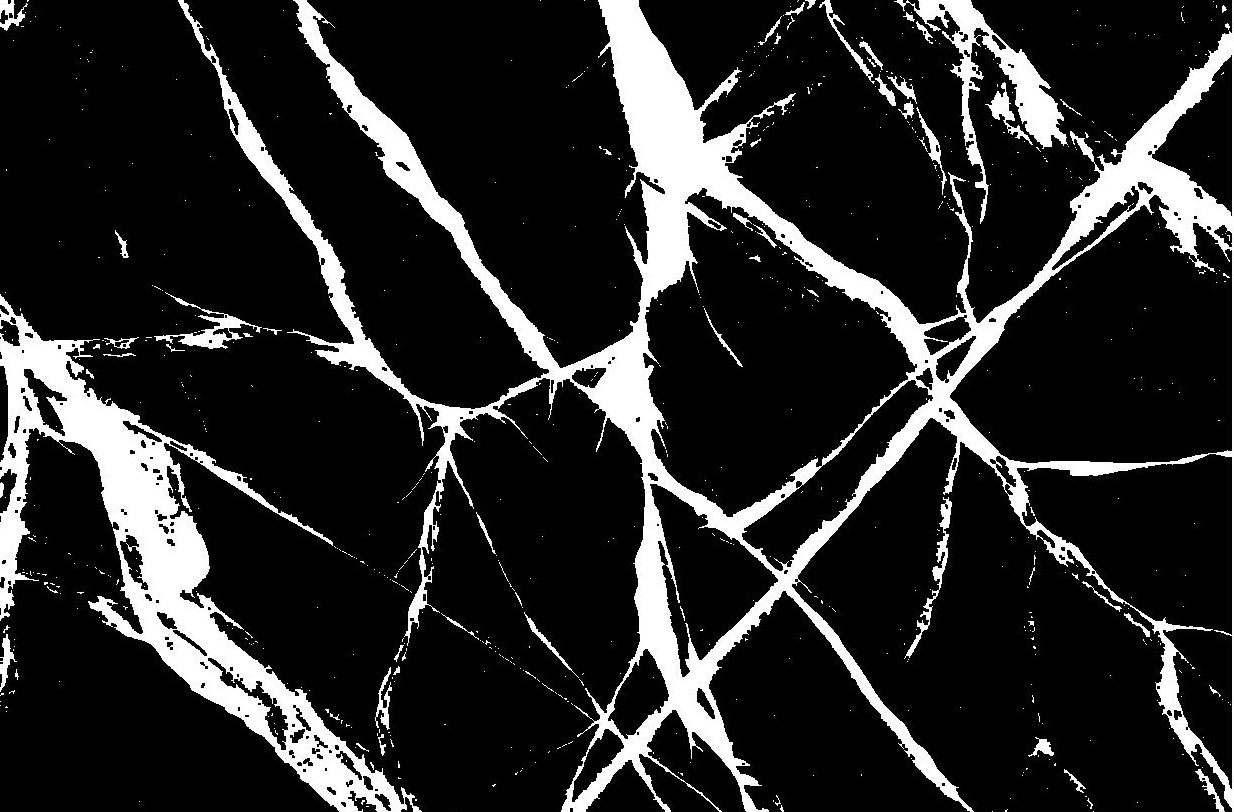
\includegraphics[width=\textwidth]{ice_close}
        \caption{Closing}
        \label{fig:ice_close}
    \end{subfigure} 
    \begin{subfigure}[b]{0.49\textwidth}
        \[
        \begin{bmatrix}
            1 & 1 & 1 & 1 & 1 & 1 & 1 & 1 & 1 \\
            1 & 1 & 1 & 1 & 1 & 1 & 1 & 1 & 1 \\
            1 & 1 & 1 & 1 & 1 & 1 & 1 & 1 & 1 \\
            1 & 1 & 1 & 1 & 1 & 1 & 1 & 1 & 1 \\
            1 & 1 & 1 & 1 & 1 & 1 & 1 & 1 & 1 \\
            1 & 1 & 1 & 1 & 1 & 1 & 1 & 1 & 1 \\
            1 & 1 & 1 & 1 & 1 & 1 & 1 & 1 & 1 \\
            1 & 1 & 1 & 1 & 1 & 1 & 1 & 1 & 1 \\
            1 & 1 & 1 & 1 & 1 & 1 & 1 & 1 & 1 
        \end{bmatrix}
        \]
        \caption{Structuring element}
        \label{fig:structuring_element}
    \end{subfigure}
    \captionsetup{format = hang}
    \caption{Effect of morphological operations on a binary image using a 9x9 square structuring element. Original image by }
    \label{fig:morphology}
  \end{figure}


